\documentclass{article}
\usepackage[utf8]{inputenc}
\usepackage{amsmath}
\usepackage{amssymb}
\usepackage{ragged2e}
\usepackage[noend, linesnumbered]{algorithm2e}
\usepackage{amsthm} 
\usepackage{listings}
\usepackage{babel}
\usepackage{graphicx}

\title{Assignment 3}
\author{Ayman Shahriar \;\; UCID: 10180260 \;\;  Tutorial: T02 }
\date{\today}

\begin{document}
\maketitle

\raggedright
\setlength{\parskip}{0.8em}  % for default spacing, set to 0em

%%%%%%%%%%%%%%%%%%%%%%%%%%%%%%%%%%%%%%%%%%%%%%%%%%%%%%%%%%%%%%%%%%%%%%%%%%

\subsection*{a)}

\textbf{i)} The sequence of vertices of G visited using a DFS traversal starting at vertex 1: [1, 2, 3, 4, 6, 5, 7, 8]

\textbf{ii)} The sequence of vertices of G visited using a BFS traversal starting at vertex 1: [1, 2, 3, 4, 6, 5, 7, 8]

\textbf{iii)} Yes, G is connected. That is because every node in G is reachable from every other node. The shortest list of edges to remove such that the graph is no longer connected is $\{(4, 6)\}$.

\textbf{iv)} Yes, G contains a cycle. For example, the path $(1, 2, 3, 1)$ is a cycle that is present in G.

\textbf{v)} No, G is not a tree. By definition, a tree is a connected, acyclic graph. Although we said that G is connected in part iii), we also mentioned that G contains a cycle in part iv). Then since G contains a cycle, G cannot be a tree.

%%%%%%%%%%%%%%%%%%%%%%%%%%%%%%%%%%%%%%%%%%%%%%%%%%%%%%%%%%%%%%%%%%%%%%%%%

\subsection*{b)}

\textbf{i)} The DFS tree of a complete graph $G = (V, E)$ will be the subgraph $G^{\prime} = (V^{\prime}, E^{\prime})$ such that:
\begin{itemize}
    \item $V^{\prime} \subset V$
    \item $(u, v) \in E^{\prime}$ $\iff$ $u,v \in V$ and $u$ is the node from which $v$ was visited the first time in the DFS.
\end{itemize}

In informal terms, the DFS tree of a complete graph G will be a "straight-line" subgraph of G that contains all it's vertices and corresponds to a simple path in G that starts with the source vertex and ends with the last vertex discovered in the DFS. And in this tree, each node and the node from which it was visited from the first time in the DFS is connected by an edge.

So as a drawing, a tree of i nodes (with n\_1 being the source vertex) would look like:

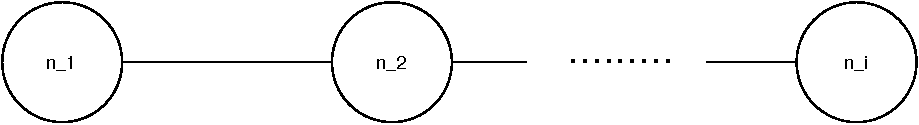
\includegraphics[scale=0.7]{draw1.pdf}

\BlankLine
\textbf{ii)} The BFS tree of a complete graph $G = (V, E)$ will be the subgraph $G^{\prime} = (V^{\prime}, E^{\prime})$ such that:
\begin{itemize}
    \item $V^{\prime} \subset V$
    \item $(s, v) \in E^{\prime}$ $\iff$ $s$ is the source vertex of the BFS and $v \in V^{\prime}-\{s\}$
\end{itemize}

In informal terms, the BFS tree of a complete graph G will be a subgraph that contains all the vertices of G and where there will be an edge between the source vertex $s$ and all the other nodes.

So as a drawing the tree of i nodes (with n\_1 being the source vertex) would look like:

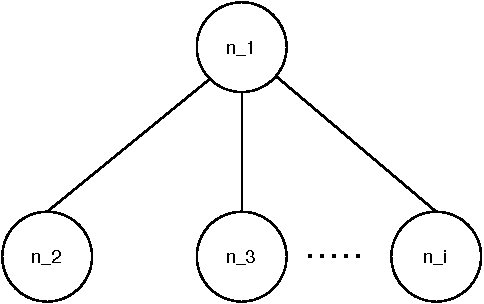
\includegraphics[scale=0.7]{draw2.pdf}

%%%%%%%%%%%%%%%%%%%%%%%%%%%%%%%%%%%%%%%%%%%%%%%%%%%%%%%%%%%%%%%%%%%%%%%%%%
\subsection*{c)}
We can store the adjacent vertices of each vertex in an array of size $n$ (where $n$ is the number of vertices of $G$). \\
So each vertex will have an array of size $n$ to store their adjacent vertices.\\ 
The $i$ nodes that are adjacent to a node will fill up the first $0, 1, 2, \dots i$ indexes of that node's array of adjacent vertices.
And as for the indexes that do not contain any vertices, we set them to a null value (for example, -1).\\ 
To keep track of how many nodes an adjacency array contains, we can use integer $S_v$ to keep track of the number of nodes in the adjacency array of node $v$.

And when initializing or modifying the adjacency arrays of each node, we have to make sure that the nodes in each array are always sorted in increasing order.

So with all these preconditions set up, this is how we can determine if the vertex $a$ is adjacent to the vertex $b$:\\
We use binary search on the adjacency array of a, searching from index 0 to index $(S_a-1)$ for the value b. If the search returns true, then $a$ and $b$ are adjacent. Otherwise, they are not adjacent.

It is common knowledge that the worst case runtime of binary search is $O(\log n)$, where n is the length of the array section being searched. Since each adjacency array will have $n-1$ vertices in the worst case, then it means that in the worst case we will have to use binary search on the entire array of length $n$.
Thus, the time to check if two vertices are adjacent is in $O(\log n)$.






%%%%%%%%%%%%%%%%%%%%%%%%%%%%%%%%%%%%%%%%%%%%%%%%%%%%%%%%%%%%%%%%%%%%%%%%%%%%

\subsection*{d)}

This claim is true. We will prove the claim using contradiction:

Suppose G is a graph with $n$ nodes, where $n$ is even. Suppose that every node of G has degree of at least $\frac{n}{2}$, but G is not connected.

Since G is not connected, there must exist two connected components $C_1$, $C_2$ in G such that no node in $C_1$ has a neighbour in $C_2$, and no node in $C_2$ has a neighbour in $C_1$.

Consider nodes $u \in C_1$ and $v \in C_2$.

Since u has degree of at least $\frac{n}{2}$, it must be connected through vertices to at least $\frac{n}{2}$ other nodes that are in $C_1$. So $C_1$ will contain at least $\frac{n}{2} +1$ nodes.

Since v has degree of at least $\frac{n}{2}$, it must be connected through vertices to at least $\frac{n}{2}$ other nodes that are in $C_2$. So $C_2$ will contain at least $\frac{n}{2} +1$ nodes.

So G will contain at least $\frac{n}{2}+1+\frac{n}{2}+1 = n+2$ nodes, which contradicts the assumption that G has $n$ nodes.

Thus, the claim is true.




%%%%%%%%%%%%%%%%%%%%%%%%%%%%%%%%%%%%%%%%%%%%%%%%%%%%%%%%%%%%%%%%%%%%%%%%%%%%

\subsection*{3a)}

Here is a precise specification of the problem:

Pre-conditions:
\begin{itemize}
    \item An undirected graph $G=(V, E)$. 
    \item $V$ will be a finite, non-empty set of vertices. 
    \item $E$ will be a finite set of edges. 
    \item Each edge is an unordered pair of distinct vertices.
\end{itemize}

Post-conditions: 
\begin{itemize}
    \item If $G$ contains a cycle, then return a linked list of nodes $C = (n_a, n_b, n_c, \dots ,n_a)$ that corresponds to a cycle in G.
    \item Otherwise if G does not contain a cycle, return an empty linked list C.
    \item G is not modified.
\end{itemize}




%%%%%%%%%%%%%%%%%%%%%%%%%%%%%%%%%%%%%%%%%%%%%%%%%%%%%%%%%%%%%%%%%%%%%%%
\subsection*{b)}
This is the pseudocode of the algorithm. It is a modified version of the BFS algorithm from slides 34-35, 58 of the set of notes titled "CPSC413-4Graphs\_ha"

\begin{algorithm}[H]
\DontPrintSemicolon
\SetAlgoLined
\SetKwProg{Fn}{Function}{}{} %% defines function
\SetArgSty{textup}  %% prevents italic text

\Fn{DFS(G = (V, E))} {
    \;
    //Preprocessing:\\
    Initialize empty linkedlist C\\ 
    \For{each vertex u in V:}{
        color[u] = white\\
        $\pi$[u] = Nil\\
    }
   \;
    \For{each vertex s in V:}{
        \If{s is white} {
            DFS-Visit(s)\\
            \If{C != empty:} {
                break
            }
        }
    }
    \;
    return C\\
}
\end{algorithm}



\begin{algorithm}[H]
\DontPrintSemicolon
\SetAlgoLined
\SetKwProg{Fn}{Function}{}{} %% defines function
\SetArgSty{textup}  %% prevents italic text

\Fn{DFS-Visit(u)} {
    \;
    color[u] = red\\
    \For{each neighbour v of u}{
        \If{color[v] == red and $\pi$[u] $\neq$ v}{
            C.add(v)\\
            Get-Cycle(u, v)\\
            \;
            //Set color of all vertices to blue\\
            \For{each vertex v in V}{
                color[v] = blue\\
            }
        }
        \;
        \If{color[v] == white}{
            $\pi$[v] = u\\
            DFS-Visit(v)\\
        }
        \;
    color[u] = blue\\
    }
}
\end{algorithm}


\begin{algorithm}[H]
\DontPrintSemicolon
\SetAlgoLined
\SetKwProg{Fn}{Function}{}{} %% defines function
\SetArgSty{textup}  %% prevents italic text

\Fn{Get-Cycle(startNode, stopNode)} {
    \If{startNode == stopNode}{
    C.add(stopNode)\\    
    }
    \;
    \Else{
        C.add(startNode)\\
        Get-Cycle($\pi$[startNode], stopNode)\\
   }
   
}
\end{algorithm}



%%%%%%%%%%%%%%%%%%%%%%%%%%%%%%%%%%%%%%%%%%%%%%%%%%%%%%%%%%%%%%%%%%%%%%%%%%%%
\subsection*{c)}
In order to detect whether a graph contains a cycle, we have made modifications to the Depth First Search algorithm from the set of slides titled "CPSC413-4Graphs\_ha". \\
To prove that our algorithm is correct, we will assume that the DFS algorithm is correct and show that our adaptations will be able to detect cycles in a graph.

\textbf{The \texttt{DFS} Function:}\\
In the \texttt{DFS} function, we initialize a linked list $C$ and return that. Assume that the \texttt{DFS-Visit} and \texttt{Get-Cycle} functions work properly. Then if the connected component of node $s$ has a cycle, \texttt{DFS-Visit(s)} will fill $C$ to contain that cycle. Since we have found a cycle (and that cycle is stored in $C$), we will break from the for loop and return $C$.

If \texttt{DFS-Visit} does not find a cycle, then $C$ will be empty, so we will keep on running \texttt{DFS-Visit} on available white nodes. From the original BFS algorithm we know that if a node is white at line 11, then it means that it's connected component has not been visited yet. So in each iteration of the for loop, the \texttt{DFS-Visit} function will check for cycles in a different connected component of the graph.

If there are no white nodes left and $C$ still empty, then it means that the graph does not contain any cycle, so we will return the empty node $C$.

\textbf{The \texttt{DFS-Visit} Function:}

Let us define the following:
\begin{itemize}
    \item \textit{$v$ is the parent of $u$}: $v$ is the node from which $u$ was visited the first time, ie. $\pi[u]$ $=$ $v$
    \item \textit{$u$ is the child of $v$}: same as $v$ is the parent of $u$, ie. $\pi[u]$ $=$ $v$
    \item \textit{$v$ is the ancestor of $u$}: in the DFS tree of $G$, $v$ is the ancestor of $u$
    \item \textit{$u$ is the descendant of $v$}: in the DFS tree of $G$, $u$ is the descendant of $v$ 
\end{itemize}

In the $DFS-Visit$ function, we check if a node $u$ has a red neighbour $v$ that is not it's parent. If $v$ is a red neighbour of $u$ and not it's parent, then according to lemma 3.6, page 85 of the textbook, it means that $v$ is an "ancestor" of $u$, but not it's direct parent.

Then since $v$ is an ancestor of $u$, but not the parent of $u$, it must mean that there exists a simple path from $u$ to $v$ of length at least 2.

And since $v$ is also a direct neighbour of $u$, it means that there is another path from $u$ to $v$ of length 1.

So if we combine these two paths, we will get a simple cycle $(v, u, n \dots, v)$ of length at least 3 (so the cycle will contain at least one node $n$ that is not $u$ or $v$).

That is why in line 6 we add $v$ to $C$ and store the rest of the cycle sequence in $C$ using the function \texttt{Get-Cycle}.

Assume the \texttt{Get-Cycle} function works properly. After calling the \texttt{Get-Cycle} function, we do not need to do anything anymore except return $C$, so we need to exit from all the \texttt{DFS-Visit} function calls. We can do this by setting the color of all nodes in the graph to blue, because the for loop does not do anything if the selected node is blue. That way once a cycle is found, each of the recursive calls of \texttt{DFS-Visit} will terminate without executing anything more in the for loop. And once the control of execution returns to the \texttt{DFS} function, it will return $C$.

\textbf{The Get-Cycle Function:}\\
As mentioned, the detected cycle will be a combination of the "short" simple path $p_1 = (v, u)$ of length 1 and the "long" simple path $p_2 = (u, n, \dots, v)$ of length at least 2 (where $n \neq u$, $n \neq v$).
So that means the detected cycle will be of the form $(v, u, n, \dots, v)$ of length at least 3, were $v$ is the only repeating vertex.

To retrieve this cycle, we first add $v$ to $C$ in line 6 of \texttt{DFS-Visit}, and then call the function \texttt{Get-Cycle} to add the "long" path from $u$ to $v$ into $C$. 

As mentioned, if a node $u$ had a red neighbour $v$, then $u$ will be a descendant of $v$ but not the direct child of $v$. This means that in order to go from $u$ to $v$ "the long way around" we will have to visit the parent node of $u$, then the parent of that node, and so on until we reach $v$.

This is what \texttt{Get-Cycle} does. Each call of \texttt{Get-Cycle} takes in a start node and a stop node. It adds the start node to $C$, and recursively calls itself with the start node replaced by it's parent. It only stops calling itself when the start node is equal to the stop node.

So if we call \texttt{Get-Cycle} with $u$ as the start node and $v$ as the stop node, it will add $u$ to $C$ and keep on adding the ancestors of $u$ to $C$ until it adds $v$.
And since we had added $v$ to $C$ at the start, it means that the sequence stored inside $C$ will be a cycle.

\textbf{Conslusion:}
Thus, we have shown that these modifications of the DFS algorithm will return a cycle in $C$ if the graph contains a cycle, otherwise it will return an empty linked list $C$.
%%%%%%%%%%%%%%%%%%%%%%%%%%%%%%%%%%%%%%%%%%%%%%%%%%%%%%%%%%%%%%%%%%%%%%%%%%%%

\subsection*{d)}
From theorem 3.11, page 11 of the textbook, we know that the Depth First search algorithm runs in $O(\vert V\vert + \vert E\vert)$. So in order to determine the runtime of our modified algorithm, we will examine the runtimes of the modified parts of the algorithm.

\textbf{Runtime of Modified DFS Function:}\\ 
We initialize an empty linked list $C$ at line 4, which takes constant time.\\ 
And we also added the steps at lines 12 and 13, which exits the for loop if $C$ is not empty. Checking if a linked list is empty and exiting a loop take constant time. 

At line 15, instead of returning the array $\pi$ we return the linked list $C$. This does not affect the runtime since returning either take constant time.

So all our modifications to the DFS function run in constant time, which means that including these modifications, the algorithm still runs in $O(\vert V\vert + \vert E\vert)$.

\textbf{Runtime of Modified DFS-Visit function}
Now let us examine the modifications of the DFS-Visit function.\\

The steps at lines 5 and 6 that we added run in constant time

Note that we call the \texttt{Get-Cycle} function at line 7. After \texttt{Get-Cycle} is returned, we set all the nodes to be blue at lines 10-11. After that, the if statement at line 5 will always be false, so the \texttt{Get-Cycle} function will not be called again. Thus, we call \texttt{Get-Cycle} at most once in this function. Note that the worst case runtime of \texttt{Get-Cycle} is $O(\vert V \vert)$ (we will prove this later).

At lines 10-11, we use a for loop to set the colour of each node to be blue. Each execution of the loop will run in $O(\vert V \vert)$.
And throughout the execution of the BFS algorithm, this loop will execute at most once.

That is because in order for this loop to execute, the if statement at line 5 has to be true, which can only happen if the color of node $v$ is red.
But this will not be possible after the for loop has executed once, because the execution of the loop set all the colours of the vertices to be blue.

%That is because after we execute this for loop, all the nodes will be blue, so the if statement at line 5 will always be false.
%Since this loop is only accessed if the statement at line 5 evaluates to true, this for loop will execute at most once.


So Get-Cycle at line 7 runs in $O(\vert V \vert)$ and the for loop at line 10 runs in $O(\vert V \vert)$, and both are executed at most once in the DFS-Visit execution.
Since $O(\vert V \vert) \subset O(\vert V\vert + \vert E\vert)$ it means that the runtime of the BFS algorithm is still in $O(\vert V\vert + \vert E\vert)$.

\textbf{Runtime of Get-Cycle Function:}\\
In the worst case, the Get-Cycle function will have to add all the nodes of the graph to $C$ (this will occur in instances where the entire graph is one large cycle).

The function will recursively call itself each time it adds a node to $C$. And the only time it will not call itself is after is has added the last available node (the stopNode).

So in the worst case, the \texttt{Get-Cycle} function will recurse $\vert V \vert-1$ times.
And except for the recursive call, all the other steps of the function run in constant time. Thus, \texttt{Get-Cycle} runs in $O(\vert V \vert)$.

Since $O(\vert V \vert) \subset O(\vert V\vert + \vert E\vert)$ it means that the runtime of the BFS algorithm is still in $O(\vert V\vert + \vert E\vert)$.

\textbf{Conclusion:}
Thus, we have shown that our modified BFS algorithm still runs in $O( m + n)$, where $m = \vert V \vert$ and $n = \vert E \vert$.

%%%%%%%%%%%%%%%%%%%%%%%%%%%%%%%%%%%%%%%%%%%%%%%%%%%%%%%%%%%%%%%%%%%%%%%%%%%%

\end{document}